%% IMPORTANT: Once working, run latex 3 times to get listoffigures to work

%% Be sure to check spelling!

%% Put **your** name and the proper due date in place

%% Note that two of the \lstinputlisting and 
%% all of the \epsfig commands are currently commented out - until the
%% files exist, processing this code without them will result in an error
%% so leave the comments until you have created the files!

\documentclass{article}
\usepackage{amsmath}    % loads AMS-Math package
\usepackage{epsfig}     % allows PostScript files
\usepackage{listings}   % allows lstlisting environment
\usepackage{moreverb}   % allows listinginput environment
\usepackage[letterpaper, margin=0.75in]{geometry}  % set paper size/margins
\usepackage{EGR103F19}  % colorful file imports

\begin{document}
\begin{center}
\rule{6.5in}{0.5mm}\\~\\
\textbf{\large EGR 103L -- Fall 2019}\\~\\
\textbf{\huge Laboratory 2 - Introduction to Python}\\~\\
***NAME (NetID)***\\
***Lab Section N, DAY TIMES***\\
***DATE DUE***\\~\\
{\small I understand and have adhered to all the tenets of the Duke
  Community Standard in completing every part of this assignment.  I
  understand that a violation of any part of the Standard on any part
  of this assignment can result in failure of this assignment, failure
  of this course, and/or suspension from Duke University.} 
\rule{6.5in}{0.5mm}\\
\end{center}
\tableofcontents
\listoffigures
\pagebreak
\section{Introduction}
% put your introduction here
\section{Data Obtained}
The three data sets from the experiments are presented in Table
\ref{DataTables}.
% see handout / Pundit page for how to get formatted numbers into tables
\renewcommand{\arraystretch}{1.4}
\begin{table}[h]
\begin{center}
\begin{tabular}{ccc}
\begin{tabular}[t]{|c|c|}\hline
\multicolumn{2}{|c|}{Beam1.dat}\\ \hline
\textbf{Mass} & \textbf{Disp.}\\
(kg) & (in)\\ \hline
         0&  5.2110e-03\\
8.1541e-01 &  8.4737e-01\\
7.9714e-01&  9.9999e-01\\ \hline
\end{tabular}
&
\begin{tabular}[t]{|c|c|}\hline
\multicolumn{2}{|c|}{Beam2.dat}\\ \hline
\textbf{Mass} & \textbf{Disp.}\\
(kg) & (in)\\ \hline
         0&  5.2110e-03\\
3.8548e-01 &  4.1535e-01\\
7.9714e-01&  9.9999e-01\\ \hline
\end{tabular}
&
\begin{tabular}[t]{|c|c|}\hline
\multicolumn{2}{|c|}{Beam3.dat}\\ \hline
\textbf{Mass} & \textbf{Disp.}\\
(kg) & (in)\\ \hline
8.1541e-01 &  8.4737e-01\\
7.9714e-01&  9.9999e-01\\ \hline
\end{tabular}
\end{tabular}
\caption{Data from Three Beam Experiments \label{DataTables}}
\end{center}
\end{table}


\section{Calculation Results}
A first-order polynomial fitting algorithm determined that 
the coefficients given in Table \ref{Coefs} 
produce the best-fit of the data to a straight line.
% replace the Greek letters with your calculations
\begin{table}[h]
\begin{center}
\begin{tabular}{r|c|c}
Data File & Compliance (m/N) & Init. Disp. (m)\\ \hline \hline
\texttt{Beam1.dat} & $\alpha$ & $\beta$ \\ \hline
\texttt{Beam2.dat} & $\gamma$ & $\delta$ \\ \hline
\texttt{Beam3.dat} & $\epsilon$ & $\zeta$ \\ \hline
\end{tabular}
\caption{Table of Compliances and Initial Displacement Values \label{Coefs}}
\end{center}
\end{table}

% \pagebreak % turn this on if it makes sense to do so by removing the first %

\section{Conclusions}
% Add your conclusions here
\pagebreak

\appendix
\section{Codes}
% Put the name of your file in the subsection name 
% and the listinginput input
% Be sure to include the community standard in codes!
% Add \pagebreaks if they make sense

% Note that _ in section names need \ in front (that is, \_)
% while _ in file names for lstinputlisting do not.

%%% Almost everything in this section is done; make sure you 
%%% understand how it works in general and be sure to 
%%% uncomment the lstinputlisting lines once you have created the files
\lstset{style=python103, language=python} 
\subsection{run\_beam1.m}
\lstinputlisting{run_beam1.py}
\pagebreak % this will make sure the second code is all on one page
\subsection{run\_beam2.m}
%\lstinputlisting{run_beam2.py}
\pagebreak  % this will make sure the third code is all on one page
\subsection{run\_beam3.m}
%\lstinputlisting{run_beam3.py}
\pagebreak  % this will start figures on a new page 
\section{Figures}
%%% Almost everything in this section is done; make sure you 
%%% understand how it works in general and be sure to 
%%% uncomment the epsfig lines once you have created the graphs
\begin{figure}[htb]
\begin{center}
%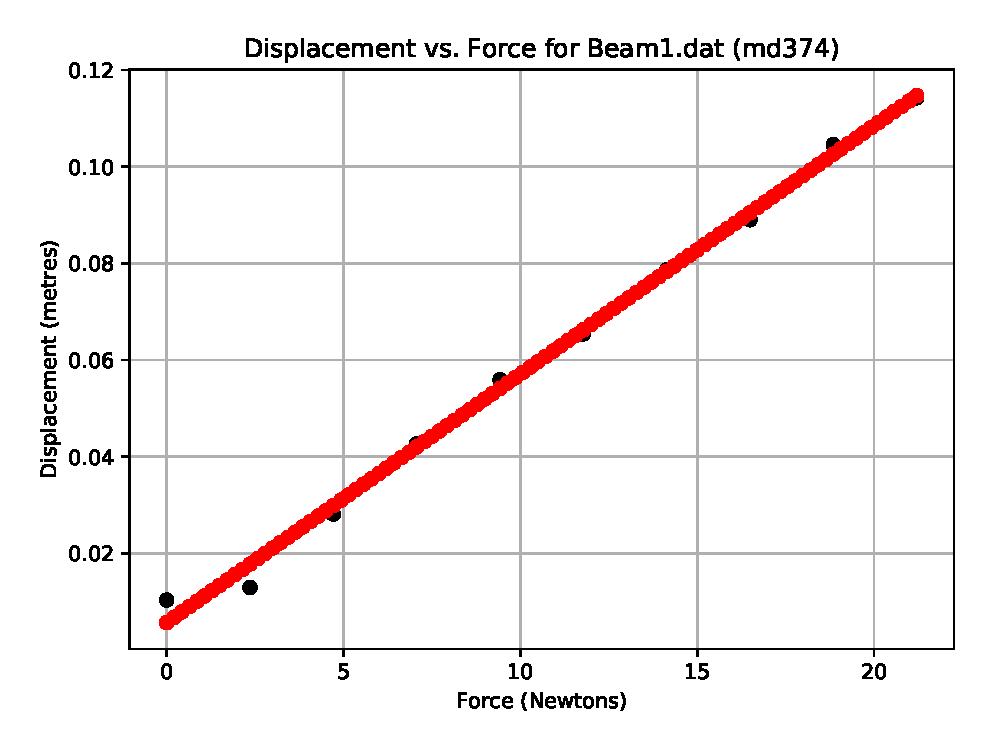
\epsfig{file=Beam1Plot.eps, width=4.5in}
\caption{Displacement vs. Force for Beam 1}
\end{center}
\end{figure}

\begin{figure}[htb]
\begin{center}
%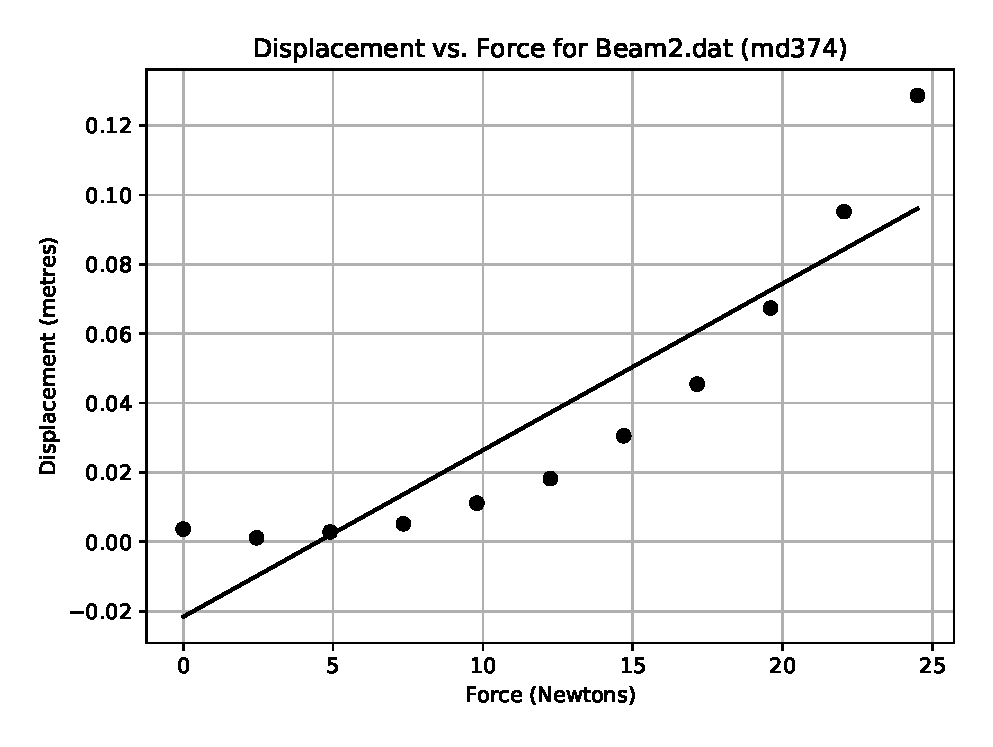
\epsfig{file=Beam2Plot.eps, width=4.5in}
\caption{Displacement vs. Force for Beam 2}
\end{center}
\end{figure}

\begin{figure}[htb]
\begin{center}
%\epsfig{file=Beam3Plot.eps, width=4.5in}
\caption{Displacement vs. Force for Beam 3}
\end{center}
\end{figure}
\end{document}
